\chapter{Calibration}

In order to achieve high fidelity imaging, any systematic offsets of the radar sensor must be compensated.
In this chapter, the systematic errors of the radar are observed and classified. With knowledge of their stability and overall characteristics,
an online calibration method is implemented and its performance analised.

\section{Stability Analysis}
The systematic errors described in section <> manifest by distorting amplitude and phase of each channel's deramped signal.
Static calibration is feasible if the systematic errors are not affected by changes of the following variables:
system restart, time elapsed since system restart, system temperature and the deramped signal's frequency.

\subsection{Setup}
The sensor is placed in a low-reflection environment and a corner reflector is placed at boresight in front of the sensor.
The time data collected in all channels is collected for a duration of two hours.
Due to the reflector's geometry, the runtime of each transmitted wavefront should be identical.
Thus, the ideal deramped signal should be of a single frequency and without inter-channel phase differences. \\

To check if the systematic offset changes on system restart, multiple restarts have to be recorded, so the experiment is repeated four times.

\begin{figure}
    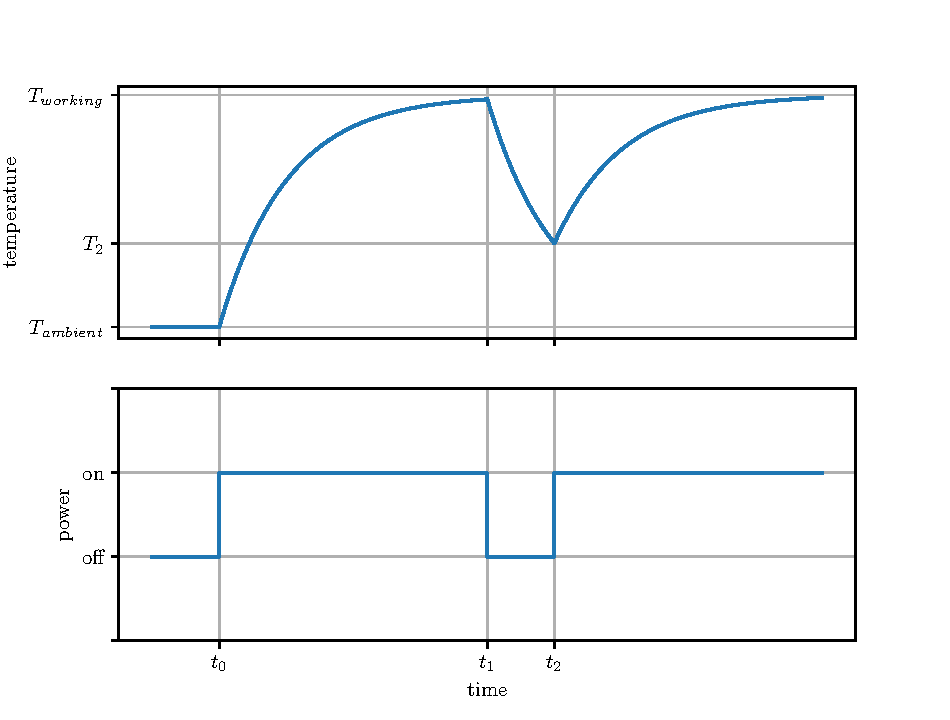
\includegraphics[width=\textwidth]{../figures/temperature.pdf}
    \caption{Expected System Temperature over Time for Interrupted Power }
    \label{fig:temperature}
\end{figure}

The system runtime and temperature cannot be considered independent variables, as illustrated in figure \ref{fig:temperature}:
the system starts at ambient temperature, heating up and approaching a stable operating temperature on turning on ($t_0$), and cooling back down after turning off ($t_1$).
The longer the runtime, the higher the temperature.

Therefore, if either one has an observable effect on the systematic offset, a different experiment has to be done where their effects are isolated.
This can be acheived by either varying the system temperature at startup (e.g. at a higher than ambient temperature at time $t_2$, achieve by a shorter cool-down interval),
or applying external heating or cooling to the system. However, change in temperature may not have an observable effect of the measured signal,
since an on-board temperature calibration is included in the AWR2243P chip.

\subsection{Results}
To briefly assess the signal quality achieved with out experiment, an arbitrary single-channel example ramp is shown in figure asdfasdf.
Visually, very low distortion to the sinusoid is visible. Looking at the spectrum of the entire signal,
the frequency peak is decently sharp, with a 3dB-width of asdfasdf and a steepness of approximately asdfasdf.

Overall, the frequency peaks location has a variance of asdfasdf, corresponding to an accuracy of asdfasdf mm. \\

Next, the deramped signal's phase and amplitude is assessed, again by calculating the DFT of each ramp.
For lack of a better comparison, offsets are defined as the difference in phase and amplitude to those exhibited by the first channel during the first ramp.
Phase and amplitude are inspected seperately.

The following figures show
\section{Calibration}
